\section{Técnicas de Agrupamento em Fluxos de Dados}

\rewrite{apresentar de outra forma (tabela?), destacar mais relevantes/importantes?}

Abordagens de agrupamento de dados são tipicamente utilizadas no aprendizado não supervisionado. Dentro da área de FD é comum verificar a falta de informação de classe, seja por conta da natureza do domínio (não existem classes definidas) ou pela dificuldade em rotular exemplos de um FD.

Independentemente dos métodos adotados, é desejável que algoritmos de agrupamento em FDs possuam a capacidade de \cite{Amini2014}: 
\begin{enumerate*}[label=\itshape\alph*\upshape)]
\item descobrir grupos de formatos arbitrários;
\item lidar com ruído;
\item realizar o agrupamento sem informação prévia sobre o número de grupos
\end{enumerate*}.

%Há diferentes técnicas para agrupamento em FD e elas podem ser divididas de acordo com a abordagem de agrupamento que seguem.

\rewrite{falar sobre propostas baseada em chunks de exemplos}

\subsection{\emph{Framework Online-Offline} (FOO) para Agrupamento em FD} \label{ChAFD:framework}

Algoritmos de agrupamento baseados em exemplos podem ser resumidos em dois passos \cite{Cao2006,Yang2006}: abstração dos dados (componente\emph{online}) e agrupamento (componente \emph{offline}), ilustrados na \autoref{Fig:onlineOffline}.

\begin{figure}[!htb]
	\centering
	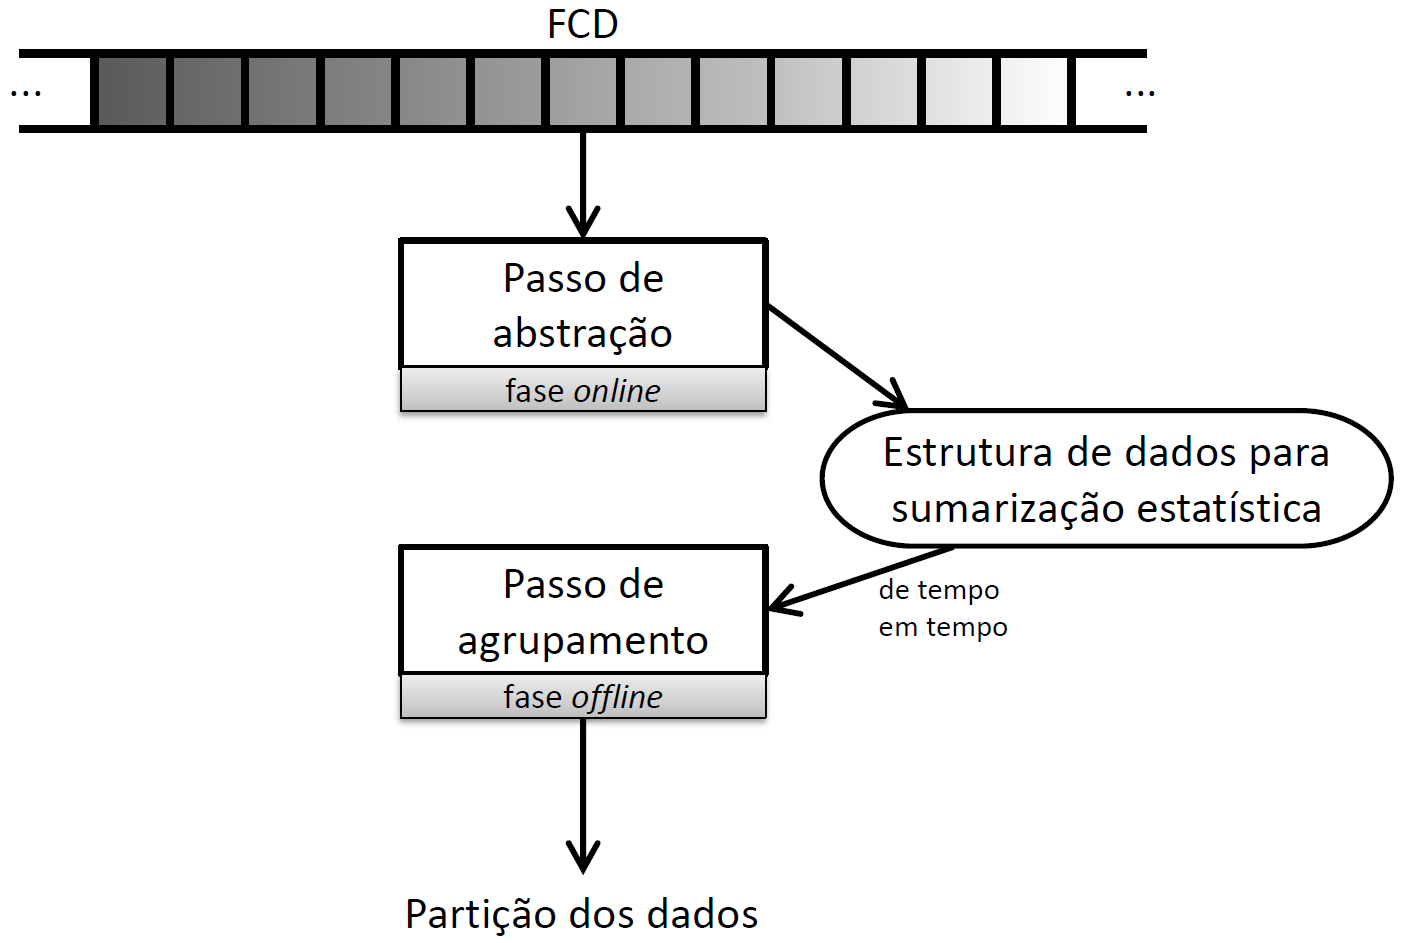
\includegraphics[width=0.7\textwidth]{figures/onlineOffline}
	\caption{\emph{Framework} \emph{online-offline} \cite{Silva2013}}\label{Fig:onlineOffline}
\end{figure}

A fase \emph{online}, abstração dos dados, sumariza os dados do FD com o auxílio de estruturas particulares para lidar com restrições de espaço e memória das aplicações FD. Essas estruturas de sumarizam os dados para preservar o significado dos objetos originais sem a necessidade de armazená-los. Estruturas frequentemente utilizadas são vetores de atributos, arranjos de protótipos e grades de dados. Essas estruturas são melhor detalhadas na \autoref{chConceitos:FD:Sumario}.

Para a contínua sumarização dos exemplos que chegam e dar maior importância aos exemplos mais recentes, uma abordagem popular é a definição de janelas temporais, como apresentado na \autoref{chConceitos:FD:Janelas}.

Durante o passo de abstração, algoritmos de agrupamento em FD devem utilizar mecanismos para detecção de \emph{outliers} que sejam capazes de diferenciar verdadeiros \emph{outliers} de evolução de grupos (\autoref{chConceitos:FD:Desvios}), uma vez que a distribuição dos dados pode variar de acordo com o tempo.

Na fase \emph{offline} é possível obter uma partição dos dados pelo passo de agrupamento. Neste momento, pode ser necessária a definição de alguns valores de entrada (número de grupos, por exemplo) para que seja possível ter uma visão geral dos grupos do FD. Algoritmos de agrupamento tradicionais podem ser utilizados considerando o conjunto de estruturas de sumarização para encontrar uma partição dos dados. O formato dos grupos encontrados está ligado ao algoritmo de agrupamento empregado, por exemplo, o $k$-\emph{means} \cite{macqueen1967} gera grupos hiperesféricos enquanto o DBSCAN \cite{Ester1996} é capaz de descobrir grupos de formatos aleatórios.

O \emph{framework} apresentado nesta seção é frequentemente utilizado para o desenvolvimento de novas técnicas de agrupamento em FD. Algumas dessas propostas são discutidas no \autoref{ChSemi}.

O \emph{ClusTree} \cite{Kranen2011}, por exemplo, é a proposta de uma estrutura hierárquica compacta e auto-adaptativa para manter sumários de FD, construindo uma hierarquia de microgrupos em diferentes níveis. Outras técnicas que seguem a abordagem hierárquica de agrupamento são o \emph{E-Stream} \cite{Udommanetanakit2007}, que possui suporte para cinco tipos de evolução em grupos (aparecimento, desaparecimento, evolução própria, mescla e divisão), e suas extensões para suporte de incerteza (valores faltantes) em FDs heterogêneos (conjuntos que combinam atributos numérico-contínuos e categóricos) \cite{Meesuksabai2011} e FDs de alta dimensão \cite{Chairukwattana2014}.

As subseções a seguir apresentam técnicas já existentes baseadas em agrupamento particional e baseado em densidade, onde é possível identificar focos de pesquisas mais recentes.

\subsection{Agrupamento Particional em FD}

Os algoritmos de agrupamento particional para FD, em sua maioria, são propostos como extensões de algoritmos de agrupamento particionais conhecidos, como $k$-\emph{means}, $k$-medóides e \emph{Affinity Propagation}.

O algoritmo \emph{CluStream} \cite{Aggarwal2003} é baseado no algoritmo $k$-\emph{means} e introduz um \emph{framework} \emph{online-offline} para agrupamento em FD que vem sendo adotado para grande parte dos algoritmos propostos recentemente. \citeonline{Yang2006} propõem uma extensão chamada \emph{HCluStream} para lidar com FDs heterogêneos.

A proposta de \citeonline{Labroche2014} está baseada no algoritmo $k$-medóides e realiza agrupamento \emph{fuzzy} de forma incremental. O trabalho de \citeonline{Lemos2013} apresenta uma técnica para geração de um classificador \emph{fuzzy} baseado em agrupamento incremental para a geração de regras que descrevem novos estados operacionais de um sistema de detecção e diagnóstico de falhas.

\citeonline{Hore2007} apresentam a proposta de uma abordagem genérica para agrupamento iterativo \emph{fuzzy}/possibilístico em FD, introduzindo equações objetivo transformadas para os algoritmo FCM \cite{Bezdek1981}, \emph{possibilitistc $c$-means} \cite{Krishnapuram1996} e Gustafson-Kessel \cite{Gustafson1978}. Outro trabalho \cite{Hore2007a} traz uma nova variante do FCM para aprendizado em FD, o \emph{Streaming} FCM, que realiza adaptação à evolução de distribuições pela utilização de uma parte do histórico de protótipos/centróides no agrupamento de \emph{chunks} de dados, conforme sua chegada. Em \cite{Hore2008} é explorada uma extensão \emph{online} para o FCM que mantém sumarização do agrupamento usando exemplos ponderados. Os exemplos ponderados obtidos pelo agrupamento de cada \emph{chunk} de dados formam um \emph{ensemble} que é transformado em um conjunto de grupos finais.

Alguns trabalhos propõem algoritmos baseados no agrupamento \emph{Affinity Propagation} (AP) \cite{Frey2007}. Usando método de passagem de mensagem, o AP escolhe, entre os exemplos disponíveis, aqueles que melhor representam o conjunto, os chamados \emph{exemplars}, que indicam os diferentes grupos dentro do conjunto de exemplos. Com os \emph{exemplars} não é necessário definir o número de grupos inicialmente.

Uma extensão do AP  para aprendizado em FD é o algoritmo \emph{Streaming} AP \cite{Zhang2008}. Esta proposta é dividida em dois passos, sendo que o objetivo do primeiro é encontrar os \emph{exemplars} ponderados dentro de um \emph{chunk} de dados por uma extensão do AP (\emph{Weighted Affinity Propagation}), enquanto o segundo visa diminuir a complexidade do modelo pela aplicação do \emph{Weighted Affinity Propagation} para o conjunto de \emph{exemplars}. Em trabalho mais recente \cite{Zhang2014}, o \emph{Streaming} AP traz melhorias como mecanismo de detecção de mudanças e adaptação do modelo da distribução dos dados.  

\subsection{Agrupamento Baseado em Densidade em FD}

Os algoritmos baseados em densidade também são utilizados como alternativa para a tarefa de agrupamento, sendo duas de suas vantagens a alta tolerância a ruído ou \emph{outliers} e a habilidade em descobrir grupos de formatos arbitrários.

As técnicas de agrupamento baseado em densidade seguem, comumente, duas abordagens que são descritas nas próximas seções e incluem exemplos de algoritmos que se encaixam nessas categorias.

\subsection{Algoritmos de Microgrupos de Densidade}

Em algoritmos de agrupamento de microgrupos de densidade, microgrupos mantêm a informação de sumarização dos exemplos e o agrupamento é realizado usando as estruturas de sinopse.

A proposta de \citeonline{Cao2006} é o algoritmo de agrupamento em FD baseado em densidade chamado \emph{DenStream}, que utiliza duas estruturas de sumarização para lidar com novas distribuições no FD, diferenciando-as de \emph{outliers}. As estruturas nomeadas \emph{core-micro-cluster} (cmc), referentes ao agrupamento em si, e \emph{pontential core-micro-cluster} (pcmc), distribuição de exemplos que representa regiões menos densas que são mantidas. O aprendizado da estrutura do FD é realizado em duas fases. Na fase \emph{online} do algoritmo, cada novo exemplo pode ser associado a um microgrupo já existente (cmc ou pcmc), de acordo com cálculo de métrica de dissimilaridade (distância Euclidiana) ou será criado um novo pcmc para o novo exemplo. Na fase \emph{offline} é aplicado o algoritmo \emph{DBSCAN} \cite{Ester1996} para determinar o grupos finais, de acordo com o conjunto de cmc. De tempos em tempos, um método de poda avalia o conjunto de pcmc para garantir que são \emph{outliers}, de acordo com a densidade, e descartá-los. O \emph{DenStream} não possui mecanismos para a eliminação de microgrupos ou para fundir dois ou mais microgrupos, o que pode ser problemático conforme o crescimento do conjunto de exemplos e limitações de espaço para armazenamento.

O \emph{DenStream} serviu de inspiração para outras técnicas que consideram situações particulares e implementam adaptações para lidar com contextos diversos. \citeonline{LiXiong2009} desenvolveram um algoritmo baseado no \emph{DenStream} para aplicações com grande volume de outliers. %O \emph{rDenStream} gera um classificador com base no resultado do agrupamento. Em um passo específico do algoritmo, dados inicialmente descartados têm a chance de ser reaprendidos. Nesta técnica os pcmc não são descartados, formando um conjunto de histórico de \emph{outliers}, o que resulta na necessidade de mais espaço para manter o histórico.
O algoritmo \emph{SDStream} \cite{Ren2009}  tem a habilidade de descobrir grupos de formatos arbitrários dentro de um modelo de janela deslizante, que permite o esquecimento progressivo dos dados antigos. %Durante o processo de aprendizagem, a distribuição dos dados mais recentes do FD é considerada e os exemplos que não mais pertencem à janela de tempo considerada são descartados. A utilização do modelo de janela deslizante permite o esquecimento dos dados antigos, pois assume-se que o interesse do usuário está na distribuição dos dados mais recentes do FD.
\emph{HDenStream} \cite{Lin2009} é um algoritmo adaptado para aprendizado em FDs com atributos heterogêneos pela inclusão de um atributo bidimensional para manter a frequência de atributos categóricos. %A técnica oferece possível solução para aplicações onde existem dados categóricos e contínuos.
O \emph{HDDStream} \cite{Ntoutsi2012} traz adaptações ao original \emph{DenStream} para melhorar o agrupamento de FDs de alta dimensão. O \emph{PreDeConStream} \cite{Hassani2012} melhora a eficiência da fase \emph{offline} do \emph{HDDStream}.

Alguns métodos híbridos utilizam conceitos do algoritmo \emph{DenStream} aliado a outras abordagens. O \emph{StreamOptics} \cite{Tasoulis2007} é um \emph{framework} baseado nos conceitos de cmc e pcmc, que utiliza o algoritmo \emph{OPTICS} \cite{Ankerst1999} para produzir visualização gráfica da estrutura do FD e sua evolução com o passar do tempo. No entanto, em nenhum momento é gerada uma partição do conjunto, então a análise do agrupamento deve ser realizada manualmente. \citeonline{Isaksson2012} propõem o algoritmo \emph{SOStream}, que detecta estrutura de FDs de rápida evolução pela adaptação automática de limiar para o agrupamento baseado em densidade. O limiar é individual por grupo e é definido automaticamente dentro do processo de agrupamento, baseado na ideia de construir vizinhanças com um mínimo de pontos, como parte da análise para criação, remoção,mescla e divisão de grupos. O algoritmo utiliza aprendizado competitivo como em \emph{Self Organizing Maps} \cite{Kohonen1982}, o que pode tornar o processo mais oneroso.

O algoritmo \emph{APDenStream} \cite{Zhang2013} baseia-se nos métodos AP e \emph{DenStream} para definição de um modelo geral que representa o FD. O algoritmo AP substitui o \emph{DBSCAN} na fase \emph{offline} do \emph{DenStream}. Baseado em trabalho anterior dos autores \cite{Forestiero2009}, FlockStream \cite{Forestiero2013} utiliza um sistema multi-agente baseado em um modelo de \emph{flocking} \cite{Kennedy2001}. Nesta técnica os agentes são microgrupos que trabalham de forma independente mas formam grupos juntos.

\subsection{Algoritmos Baseados em Densidade e Grades}

Em se tratando de agrupamento não supervisionado de FDs é possível identificar recente tendência no investimento de abordagens baseadas em grades e densidade \cite{Amini2011,Amini2014}.

%Grande parte das técnicas de agrupamento baseadas em grade e densidade seguem o fOO, mapeando os exemplos em células do espaço de atributos (grades) que são agrupadas de acordo com suas densidades. 
Uma das primeiras tentativas de associar os dois métodos foi o trabalho de \citeonline{Gao2005}, que propõe um algoritmo de agrupamento incremental de passagem única usando células do espaço de atributos (grades) densas que são consideradas em uma fase de agrupamento caso tenham valor de densidade acima de um limiar pré-definido.

O \emph{D-Stream} \cite{Chen2007, Tu2009} é uma proposta de agurpamento em tempo real baseado em grades, apoiado no fOO. Na fase \emph{online} acontece a leitura de um novo exemplo e seu mapeamento na grade. Na fase \emph{offline} os grupos são criados e ajustados em intervalos. No primeiro ciclo cada grade considerada densa é associada a um grupo distinto, nos intervalos seguintes os grupos são ajustados. O ajuste de grupos acontece por meio da identificação de grades densas e esparsas: grades densas são mescladas a grades vizinhas, formando um grupo; caso contrário a grade é removida do grupo. O método, que agrupa os exemplos em tempo real, inclui mecanismos para decaimento de densidade com a passagem do tempo, detecção de evolução de comportamento e tratamento de \emph{outliers}.

\rewrite{é aqui que eu comento do problema das grades? Tamanho da grade (como dividir o espaço), número de dimensões/atributos (grades esparsas > grades densas, mais oneroso para manter em memória e fase offline (volume de grade e verificação de grupos)}

\rewrite{O D-Stream é o principal baseado em grade e densidade, os outros podem aparecer somente na tabela, se for o caso de mencionar}

%Algumas extensões para o \emph{D-Stream I} são propostas. \citeonline{Jia2008} propuseram um modelo que melhora a qualidade dos grupos pela detecção dos pontos limites de uma grade. A extensão \emph{D-Stream II} \cite{Tu2009} inclui uma restrição de atração entre grades para a mesclagem e composição de um grupo na fase \emph{offline}. A atração entre grades é verificada pela construção de hipercubos centrados nos exemplos de uma grade, considerando cada atributo do FD, a fim de estabelecer um volume para a grade, que será utilizada para verificar se duas grades devem ou não ser mescladas em um mesmo grupo.

%Ao realizar agrupamento baseado em grades, quanto maior a dimensão do conjunto de dados, maior o número de grades vazias. Pensando nisso, \citeonline{Ren2011} propõem o algoritmo \emph{PKS-Stream} para conjuntos de alta dimensão. A técnica possui uma estrutura de árvore para manter as grades não-vazias e suas relações. À chegada de um novo exemplo, o algoritmo verifica as estruturas de sumarização de grade para ver se o exemplo pertence a alguma das grades existentes na estrutura de árvore. Caso não seja verdadeiro, um novo elemento de sumarização de grade é criado. De tempo em tempo, a árvore é ajustada, pela remoção de grades esparsas, e os grupos são formados de acordo com a densidade das grades vizinhas. O \emph{PKS-Stream I} \cite{Zhang2012a} é uma versão otimizada do \emph{PKS-Stream} quanto à seleção de período para detecção de densidade, identificação e remoção esporádica de grades.

%\emph{DCUStream} \cite{Yang2012} é um algoritmo baseado em densidade e grades para aprendizado em FDs com dados incertos. A proposta introduz o conceito de \emph{core dense grid} que é uma grade densa com vizinhos esparsos, usados no momento de agrupamento na fase \emph{offline}, quando os vizinhos esparsos são considerados ruído. O processo de busca pelos \emph{core dense grids} e seus vizinhos pode ser bastante lento.

%A proposta do algoritmo \emph{DENGRIS-Stream} \cite{Amini2012} realiza o agrupamento dentro de um modelo de janela deslizante, na tentativa de capturar a distribuição mais recente dos dados. É a primeira proposta para agrupamento baseado em densidade e grades que considera o modelo de janela deslizante.

%\emph{ExCC} \cite{Bhatnagar2013} é um algoritmo de agrupamento baseado em densidade e grades que tem como foco o aprendizado em FDs heterogêneos. O algoritmo é robusto, adaptando-se a mudanças na distribuição dos dados e detectando \emph{outliers} com rapidez. O algoritmo implementa um mecanismo para garantir o curso de novos grupos descobertos.

Pela revisão aqui exposta, pode-se verificar que é crescente o número de novas propostas para agrupamento em FDs, em especial aquelas que utilizam abordagem baseada em densidade e outras abordagens capazes de lidar com o surgimento e desaparecimento de grupos de forma simples.

No entanto, neste tipo de aprendizado, é ignorada qualquer informação prévia que possa existir a respeito da distribuição dos dados. O investimento em novas propostas para aprendizado semissupervisionado em FD também cresceu nos últimos anos, como pode ser inferido pelas técnicas apresentadas na próxima seção.

\section{Agrupamento Fuzzy em Fluxo de Dados}

O método não supervisionado de agrupamento \emph{Single Pass Fuzzy C Means} (SPFCM) \cite{Hore2007b} tem como objetivo oferecer uma alternativa ao agrupamento FCM para conjuntos de dados cujo grande tamanho impede seu armazenamento total em memória para a aplicação do processo de agrupamento. A técnica parte do princípio de que os dados do conjunto estão disponíveis em partes, nomeadas \emph{chunks}, às quais são processadas pelo algoritmo WFCM. 

O \autoref{algo:SPFCM} apresenta os passos gerais para a proposta. Quando chega o primeiro \emph{chunk} todos os exemplos possuem peso de valor 1 (um). Após a aplicação do WFCM calcula-se o peso para cada centróide obtido, com base na matriz de pertinência. Os centróides serão adicionados ao próximo \emph{chunk} de novos exemplos e o agrupamento WFCM é aplicado ao conjunto resultante dessa união.

\begin{algorithm2e}[!htb]
	\SetAlgoLined
	\Entrada{$E$, $k$, $m$, $n_{s}$}
	\Saida{$U$, $C$}
	\Inicio{
		$U = $ geraMatrizPertinênciaAleatória()\;
		$C = $ geraCentróidesIniciais($E$, $U$)\;
		$E' = $ gerarSubconjuntosExemplos($E$, $n$)\;
		$w = 1_{n_{s}}$\;
		$U, C = $ WFCM($E'[1]$,$k$,$m$,$w$)\;
		PAREI AQUI \;
		\Enqto{$\epsilon > \xi$}{
			atualizarMatrizPertinência($U$)\;
			$C'= C$\;
			atualizarCentróides($C$)\;
			$\epsilon = max_{1 \leq i \leq k}\{\| c_{i} - c'_{i} \|^{2}\}$\;
		}
	}
	\caption{\emph{Single-Pass Fuzzy} $C$-\emph{Means} (SPFCM) \cite{Hore2007b}} \label{algo:SPFCM}
\end{algorithm2e}

%O vetor $w$ é um conjunto pesos $\{w_{1}, w_{2}, ..., w_{n}\}$, onde $w_{j} \geq 0$ determina a influência de cada exemplo $e_{j}$ para o processo de agrupamento.

%As atualizações para a matriz de pertinência seguem a Equação \ref{eq:fcmAtualizaU} e geração inicial e atualização dos centróides é calculada pela Equação \ref{eq:spfcmAtualizaW} e a

%\begin{equation}
%	c_{i} = \frac{\sum_{j=1}^{n} w_{j}u_{ij}^{m}e_{j}}{\sum_{j=1}^{n} w_{j}u_{ij}^{m}}
%	\label{eq:spfcmAtualizaW}
%\end{equation}

O SPFCM contempla a dificuldade de armazenamento de exemplos, processando \emph{chunks} do conjunto e eliminando os exemplos logo após a obtenção dos centróides ponderados. No entanto, é uma técnica que considera que a distribuição dos dados é estática, o que deixa de lado a característica mutável do contexto de FD.

Os autores do SPFCM propõem, então, uma variação do algoritmo\cite{Hore2007} que inclui um mecanismo para lidar com o aspecto não estacionário dos FD. Nesta nova técnica, a partir do segundo \emph{chunk} de dados, os pesos dos centróides são calculados a partir da matriz de pertinência para os exemplos novos apenas, desconsiderando os centróides ponderados, que servem apenas como histórico de agrupamentos anteriores.

A técnica variante do SPFCM é capaz de lidar com quantidades diferentes de histórico, incorporando ao \emph{chunk} de novos exemplos $h$ conjuntos de centróides ponderados obtidos anteriormente. Uma das dificuldades nessa estratégia é determinar o valor de $h$, uma vez que essa definição depende do domínio ao qual é aplicado o agrupamento.

Outra complicação de estratégias baseadas no SPFCM é a definição prévia de um número fixo de grupos, pois, uma vez que um FD é mutável de acordo com o tempo pode ocorrer o aumento ou diminuição no número de grupos. Outro obstáculo: identificação de grupos de formato arbitrário (?)

\rewrite{
número fixo de grupos

sumarização por protótipos - centróides ponderandos (ponderação baseada na matriz de pertinência)

histórico - união de $h$ conjuntos de centróides ao novo \emph{chunk de exemplos}
}